\chapter{Introduction}

MeDSpace D2RMap is a declarative language to describe mappings between relational database schemas and OWL ontologies. The language is a derived work of the D2R Map language designed by Chris Bizer \cite{D2RMap}. As D2RMap is licensed under GNU LGPL v.2.1, this derived work is also licensed under GNU LGPL v.2.1 
\footnote{\url{http://www.gnu.de/documents/lgpl-2.1.en.html}}. 

MeDSpace D2RMap is tailored to the needs for the MeDSpace dataspace and thus some language features were removed from the original D2RMap language and other features  were added.

This document defines the syntax and semantics of the MeDSpace D2R Map language and mentions the
changes in regards to the original D2R Map language where it is needed.

The next section is basically adopted from the original D2R Map language specification \footnote{\url{http://wifo5-03.informatik.uni-mannheim.de/bizer/d2rmap/D2R\_language\%20specification.pdf}}
. The concepts have barely changed, only the language terminology and some details have changed.

\section{The D2R Mapping Process}

The D2R mapping process executed by the D2R wrapper has four logical steps:

\begin{enumerate}  
	\item Selection of a record set from the database using SQL 
	\item Grouping of the record set by the \textit{resourceIdColumns} \footnote{resourceIDColumns is an attribute of the d2r:ClassMap element}
	columns. 
	\item Creation of class instances and identifier construction. 
	\item Mapping of the grouped record set data to instance properties.
\end{enumerate}

\begin{figure}[H]
	\begin{center}
		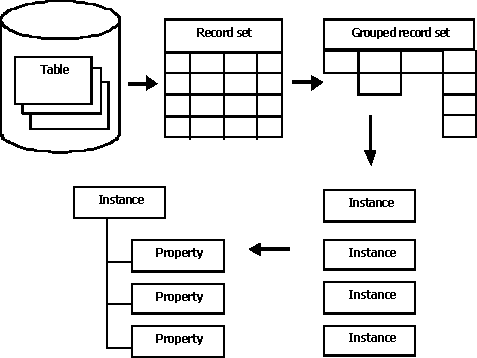
\includegraphics [width=0.75\textwidth]{../images/MappingProcess.pdf}
	\end{center}
	\caption{The MeDSpace D2R mapping process}
	\label{MappingProcessFigure}
\end{figure}

For each class or group of similar classes a record set is selected from the
database. Second, the record set is grouped according to the resourceIDColumns columns of
the specific d2r:ClassMap. Then the class instances are created and assigned an URI identifier. Blank Node creation is currently not supported, as it is not needed in the MeDSpace dataspace. Finally, the instance properties are created using
datatype and object property bridges.
The division between step three and four allows references to other instances dynamically created in the mapping process.

\chapter{Language Specification}

A MeDSpace D2R Map is a well-formed XML document. It's structure is defined by the accompanying \textit{Medspace{\_}D2RMap.xsd} file. The elements of the MeDSpace D2R Map belong to the namespace
\begin{center}
	\textbf{http://www.medspace.com/D2Rmap}
\end{center}

\section{Root Element: Map}
\textbf{Description:} \newline
Root element of the D2R-Map

\textbf{Attributes:} \newline
\BeginAttribute[xmlns, \emph{required}]
MeDSpace D2R namespace declaration.
\EndAttribute

\textbf{Sub Elements:} \newline
\BeginAttribute[DBConnection, \emph{required}]
Has to occur has the first element and it may occur only once. 
\EndAttribute
\BeginAttribute[OutputFormat, \emph{required}]
Has to occur after the DBConnection element and it may occur only once. 
\EndAttribute
\BeginAttribute[Index, \emph{optional}]
It may occur only once and has to be stated after the OutputFormat element. 
\EndAttribute
\BeginAttribute[Namespace, \emph{optional}]
Can occur any number of times
\EndAttribute
\BeginAttribute[ClassMap, \emph{optional}]
Can occur any number of times
\EndAttribute

\begin{ExampleBox}
	<d2r:Map xmlns:d2r="http://www.medspace.com/D2Rmap">
		\begin{indention}{1cm}
		\XMLComment{DBConnection element is required} \newline
		<d2r:DBConnection></d2r:DBConnection>
		
		\XMLComment{OutputFormat element is required} \newline
		<d2r:OutputFormat></d2r:OutputFormat>
		
		\XMLComment{The Index element is optional}\newline
		<d2r:Index></d2r:Index>

		\XMLComment{Than follows an optional list of namespaces and class maps in any order}\newline
		<d2r:Namespace></d2r:Namespace>\newline
		<d2r:ClassMap></d2r:ClassMap>\newline
		<d2r:ClassMap></d2r:ClassMap>\newline
		<d2r:Namespace></d2r:Namespace>
		\begin{indention}{2cm}
			\ldots
		\end{indention}		
		
		\end{indention}
	</d2r:Map>
\end{ExampleBox}


\section{Top-Level-Elements}